%!TEX program = xelatex
\documentclass{article}
\usepackage{amsthm,amsmath,amssymb}
\usepackage[UTF8]{ctex}
\usepackage[tc]{titlepic}
\usepackage{titlesec}
\usepackage{cite}
\usepackage{fancyhdr}
\usepackage{booktabs}
\usepackage{graphicx}
\usepackage{subfigure}
\usepackage{float}
\usepackage{geometry}
\usepackage[section]{placeins}
\usepackage{makeidx}
\usepackage{mathrsfs}
\usepackage{color}
\usepackage{ulem}
\usepackage{enumitem}
\geometry{a4paper,scale=0.8}
\pagestyle{fancy}

\usepackage{hyperref}
\hypersetup{hypertex=true, colorlinks=true, linkcolor=blue, anchorcolor=blue, citecolor=blue}

\usepackage{listings}
\definecolor{dkgreen}{rgb}{0,0.6,0}
\definecolor{gray}{rgb}{0.5,0.5,0.5}
\definecolor{mauve}{rgb}{0.58,0,0.82}
\lstset{frame=tb,
  language=Python,
  aboveskip=3mm,
  belowskip=3mm,
  showstringspaces=false,
  columns=flexible,
  basicstyle={\small\ttfamily},
  numbers=left,%设置行号位置none不显示行号
  %numberstyle=\tiny\courier, %设置行号大小
  numberstyle=\tiny\color{gray},
  keywordstyle=\color{blue},
  commentstyle=\color{dkgreen},
  stringstyle=\color{mauve},
  breaklines=true,
  breakatwhitespace=true,
  escapeinside=`,%逃逸字符(1左面的键),用于显示中文例如在代码中`中文...`
  tabsize=4,
  extendedchars=false %解决代码跨页时,章节标题,页眉等汉字不显示的问题
}

\lhead{第 1 次作业\\\today}
\chead{中国科学技术大学\\	DS4001 人工智能原理与技术}

\rhead{Homework 1\\ {\CTEXoptions[today=old]\today}}
\newcommand{\upcite}[1]{\textsuperscript{\cite{#1}}}

\titleformat*{\section}{\bfseries\Large}
\titleformat*{\subsection}{\bfseries\large}

\title{\bfseries 第一次作业(搜索问题)}
\author{崔士强  \quad  PB22151743}

\begin{document}
\maketitle
\textcolor{red}{\textbf{本次作业需独立完成,不允许任何形式的抄袭行为,如被发现会有相应惩罚。在上方修改你的姓名学号,说明你同意本规定。}}
% \clearpage

\section*{问题0:引入(30 分)}
\subsection*{1.最短路径问题(12分)}
\subsubsection*{a.回答问题(2分)}
\[\mathcal{D}_1 \circ d_s(v_2) = min_{v_1}\{d_s(v)+w_{v_1v_2}\} = 10 \]

\subsubsection*{b.证明(2分)}

在
\[d_s(v_k) = min_{i \in [n]}\{d_s(v_i) + w_{v_kv_i}\}\]
中,若$i \geq k$,则有$LHS > RHS$,与$d_s(v_k) \leq d_s(v_{k+1})$矛盾. 
则$i<k$,$RHS = \mathcal{D}_k \circ d_s(v_k)$.

\subsubsection*{c.证明(4分)}
定义
\[d(u) = min_{v \in S}\{d_s(v)+w_{vu}\}\]
其中$S$为已被选择的顶点集.
每轮更新即为:
\[min_{u \in V-S}\{\mathcal{D}_k \circ d(u)\} = min_{u \in V-S}\{d(u)\} = d_s(v_k)\]
也就是说,第$k$次执行算子一定能找到距源点第$k$近的点以及它到源点到最短距离,执行n次后整张图的搜索便可完成.


\subsubsection*{d.回答问题(2分)}
$\mathcal{D}_k$表示在距源点前$k$近的点(而不是所有点)当中寻找到目标点距离最短的路径. 从而
免去了对其余点的搜索,本质上是因为剩余的这些点到源点距离比目标点更长,最短路径不可能经过这些点.

\subsubsection*{e.证明(2分)}
如果 
\[d_s(u) \neq min_{v \in V}\{d_s(v)+w_{vu}\}\]
即$\exists v_0,\ s.t.\ d_s(v_0)+w_{v_0u}<d_s(u)$. 此时从源点到$v_0$的最短路径加上边$v_0u$为$u$的一条更短的路径,所以上面的假设不成立.

\subsection*{2.A*算法,判断对错并说明原因(10分)}

\begin{enumerate}
    \item[a] 正确. 此时选择结点的依据即为$d(u)$,与Dijkstra算法等价.
    \item[b] 正确. $h(u)$可能影响被选择的节点,从而影响对邻接节点的更新.
    \item[c] 错误. 从Algorithm 1 Line 4可以看出,所有的$d(u)$归根结底都是多次增加某条边权值的结果,这些边首尾相连的路径长度即为$d(u)$
    \item[d] 正确. 算法需要遍历所有顶点,在最坏情况下,每条边至少会被考察一次来更新顶点的$d$值。如果使用最小堆作为优先队列的数据结构,那么对于$m$条边,每次插入和删除的操作是$O(\log n)$。
    \item[e] 错误. $A^*$算法与Dijkstra算法等价当且仅当$h(u)=0$,然而当$h(u)$的大小排序与$d(u)$相同时也满足条件.
\end{enumerate}

\subsection*{3.网格城市(8 分)}

\subsection*{a.回答问题(8分)}
先沿$y$轴走到$(0, n)$, 再沿水平方向走到$(m, n)$,成本为$n+m+\frac{\left(1+m\right)m}{2}$.
并且没有其他最短路径.



\section*{问题1:查找最短路径(12分)}
\subsection*{a.代码实现ShortestPathProblem部分(8分)}
% 将submission.py相应部分粘贴到对应位置
\begin{lstlisting}
class ShortestPathProblem(SearchProblem):
    """The illustration and __init___ part is ommited here."""

    def startState(self) -> State:
        # BEGIN_YOUR_CODE (our solution is 1 line of code, but don't worry if you deviate from this)
        return State(self.startLocation)
        # END_YOUR_CODE

    def isEnd(self, state: State) -> bool:
        # BEGIN_YOUR_CODE (our solution is 1 line of code, but don't worry if you deviate from this)
        return self.endTag in self.cityMap.tags[state.location]
        # END_YOUR_CODE

    def successorsAndCosts(self, state: State) -> List[Tuple[str, State, float]]:
        # BEGIN_YOUR_CODE (our solution is 7 lines of code, but don't worry if you deviate from this)
        return_list = []
        for succ_location in self.cityMap.distances[state.location]:
            cost = self.cityMap.distances[State.location][succ_location]
            return_list.append((succ_location, State(succ_location), cost))
        return return_list
        # END_YOUR_CODE
\end{lstlisting}

\subsection*{b.路线可视化(4分)}
\begin{figure}[H]
    \centering
    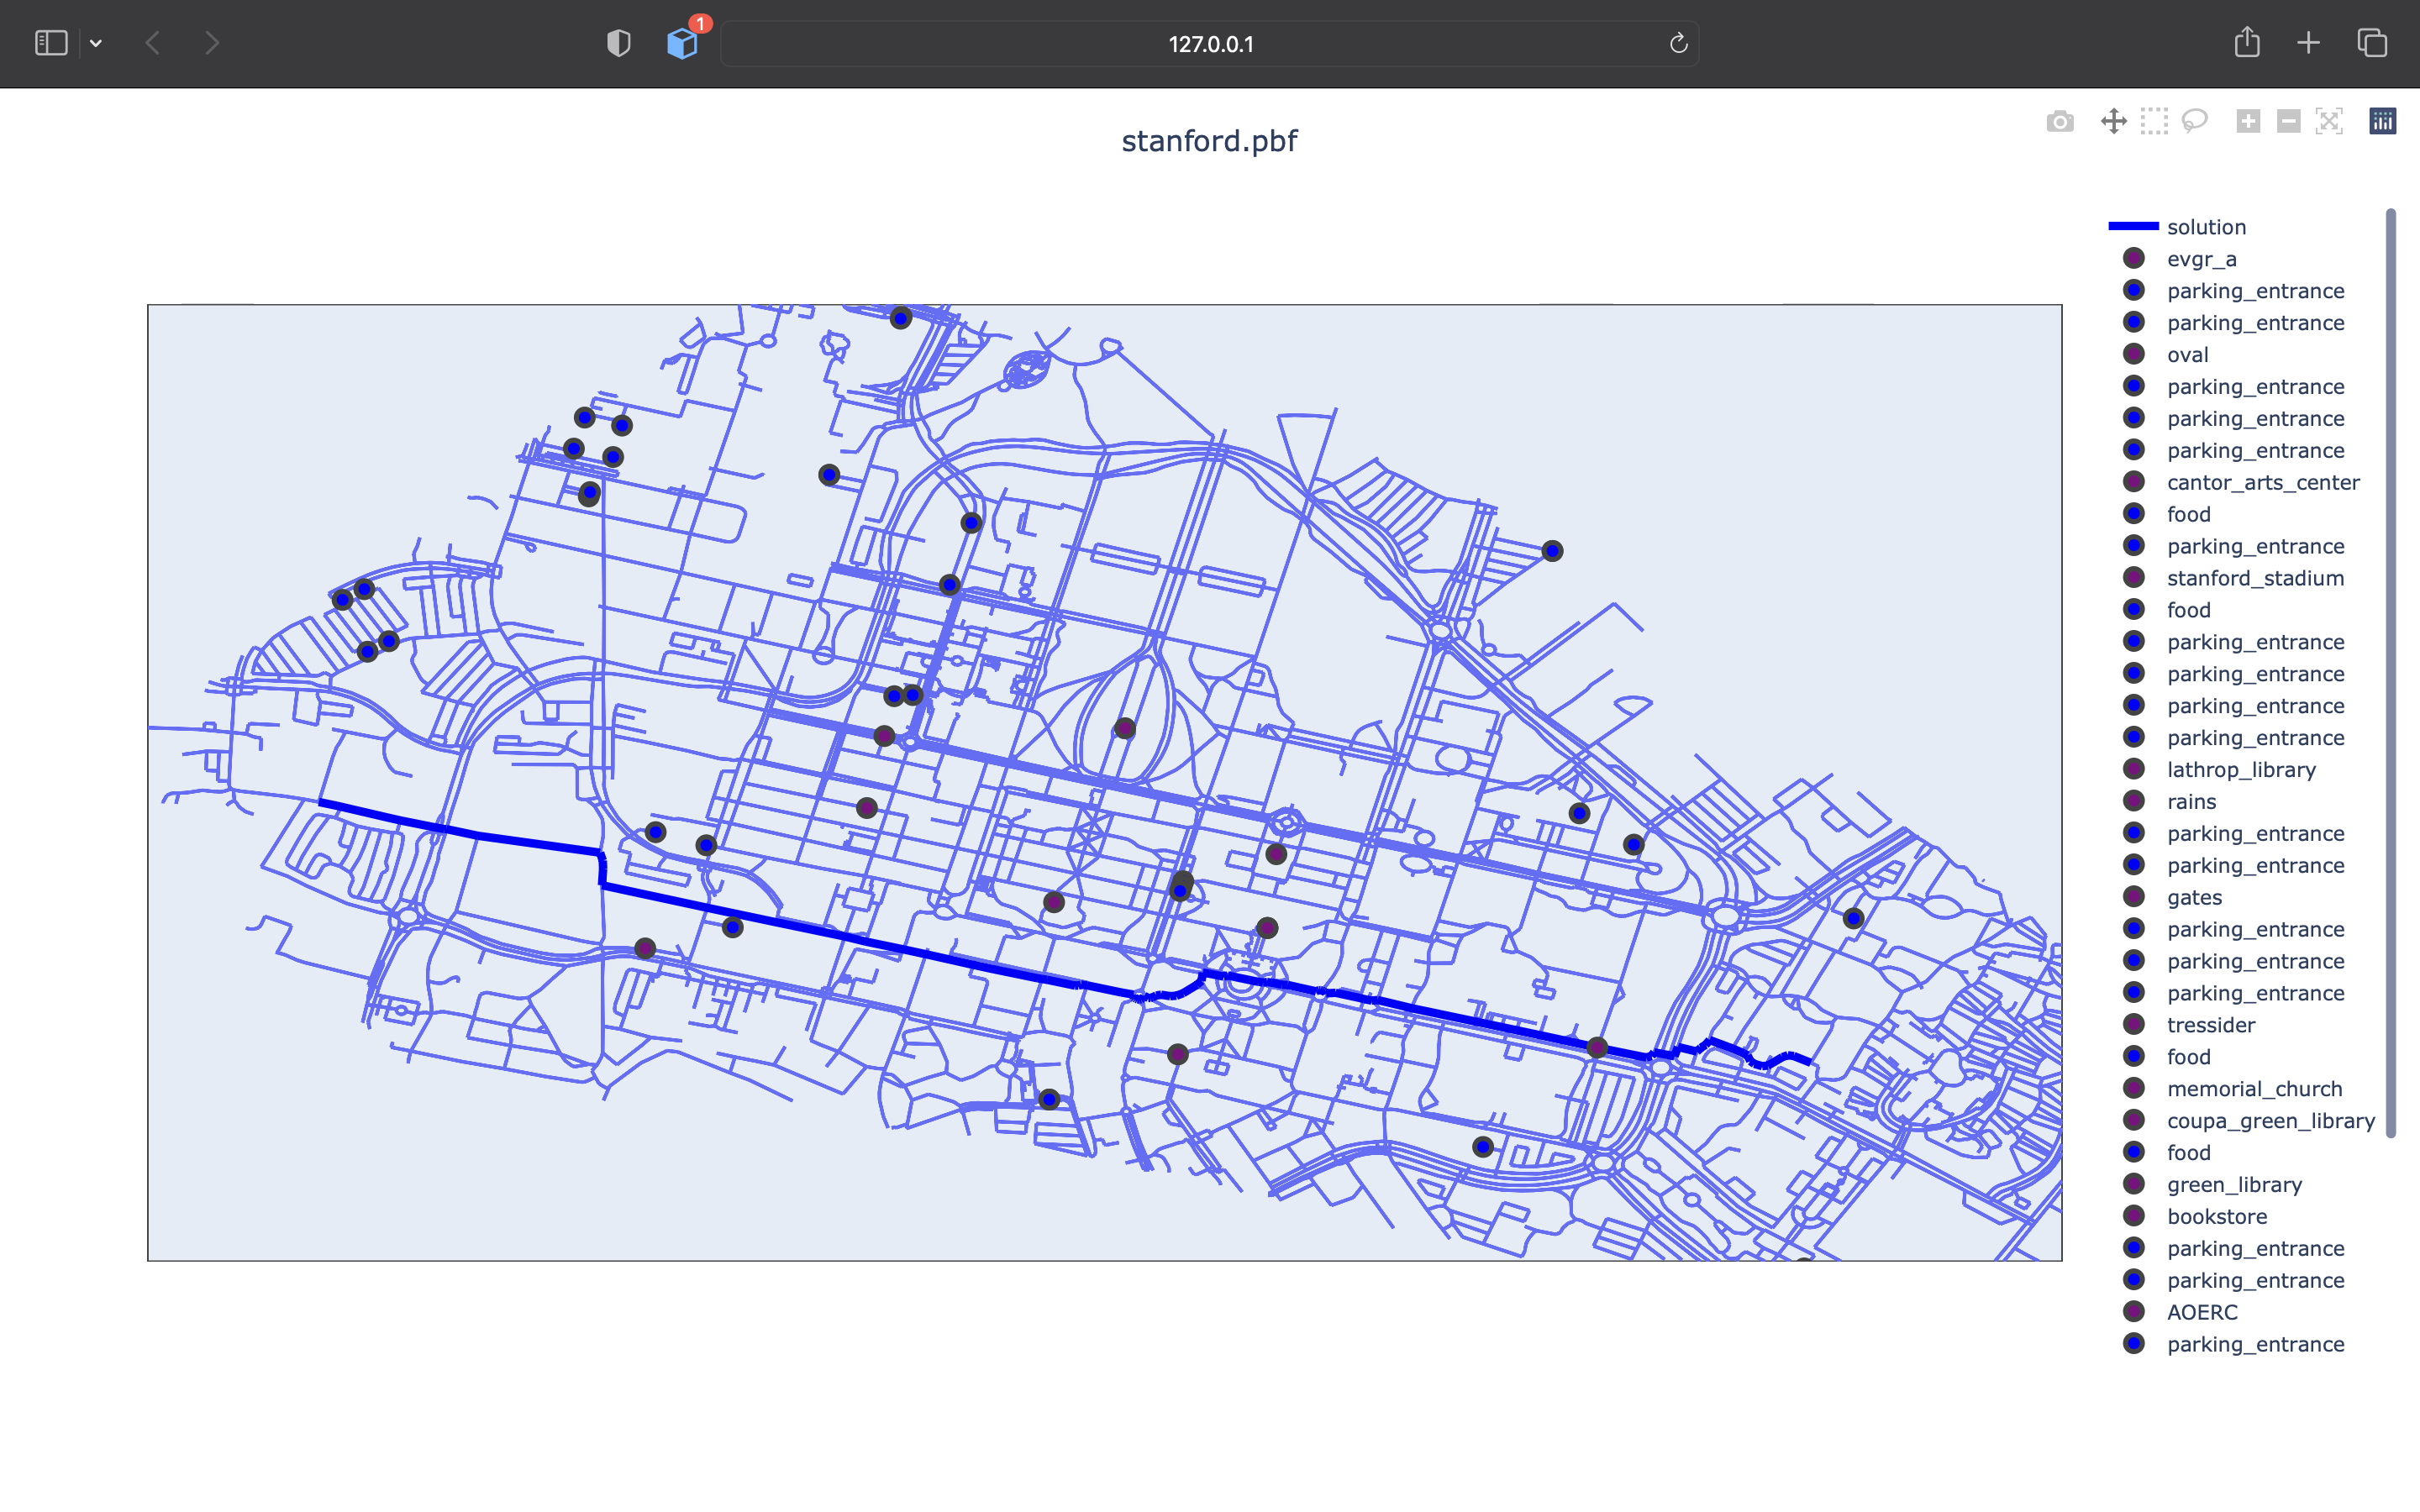
\includegraphics[width=10cm]{pics/long.png}
    \caption{startLocation='65565059', endTag="label=9384099472"}
\end{figure}

可以看到这个路线穿过了大半个校园. 这个系统对校园旅行很有帮助,可以找到起始点到任意符合要求的点的最短路径.

\begin{figure}[H]
    \centering
    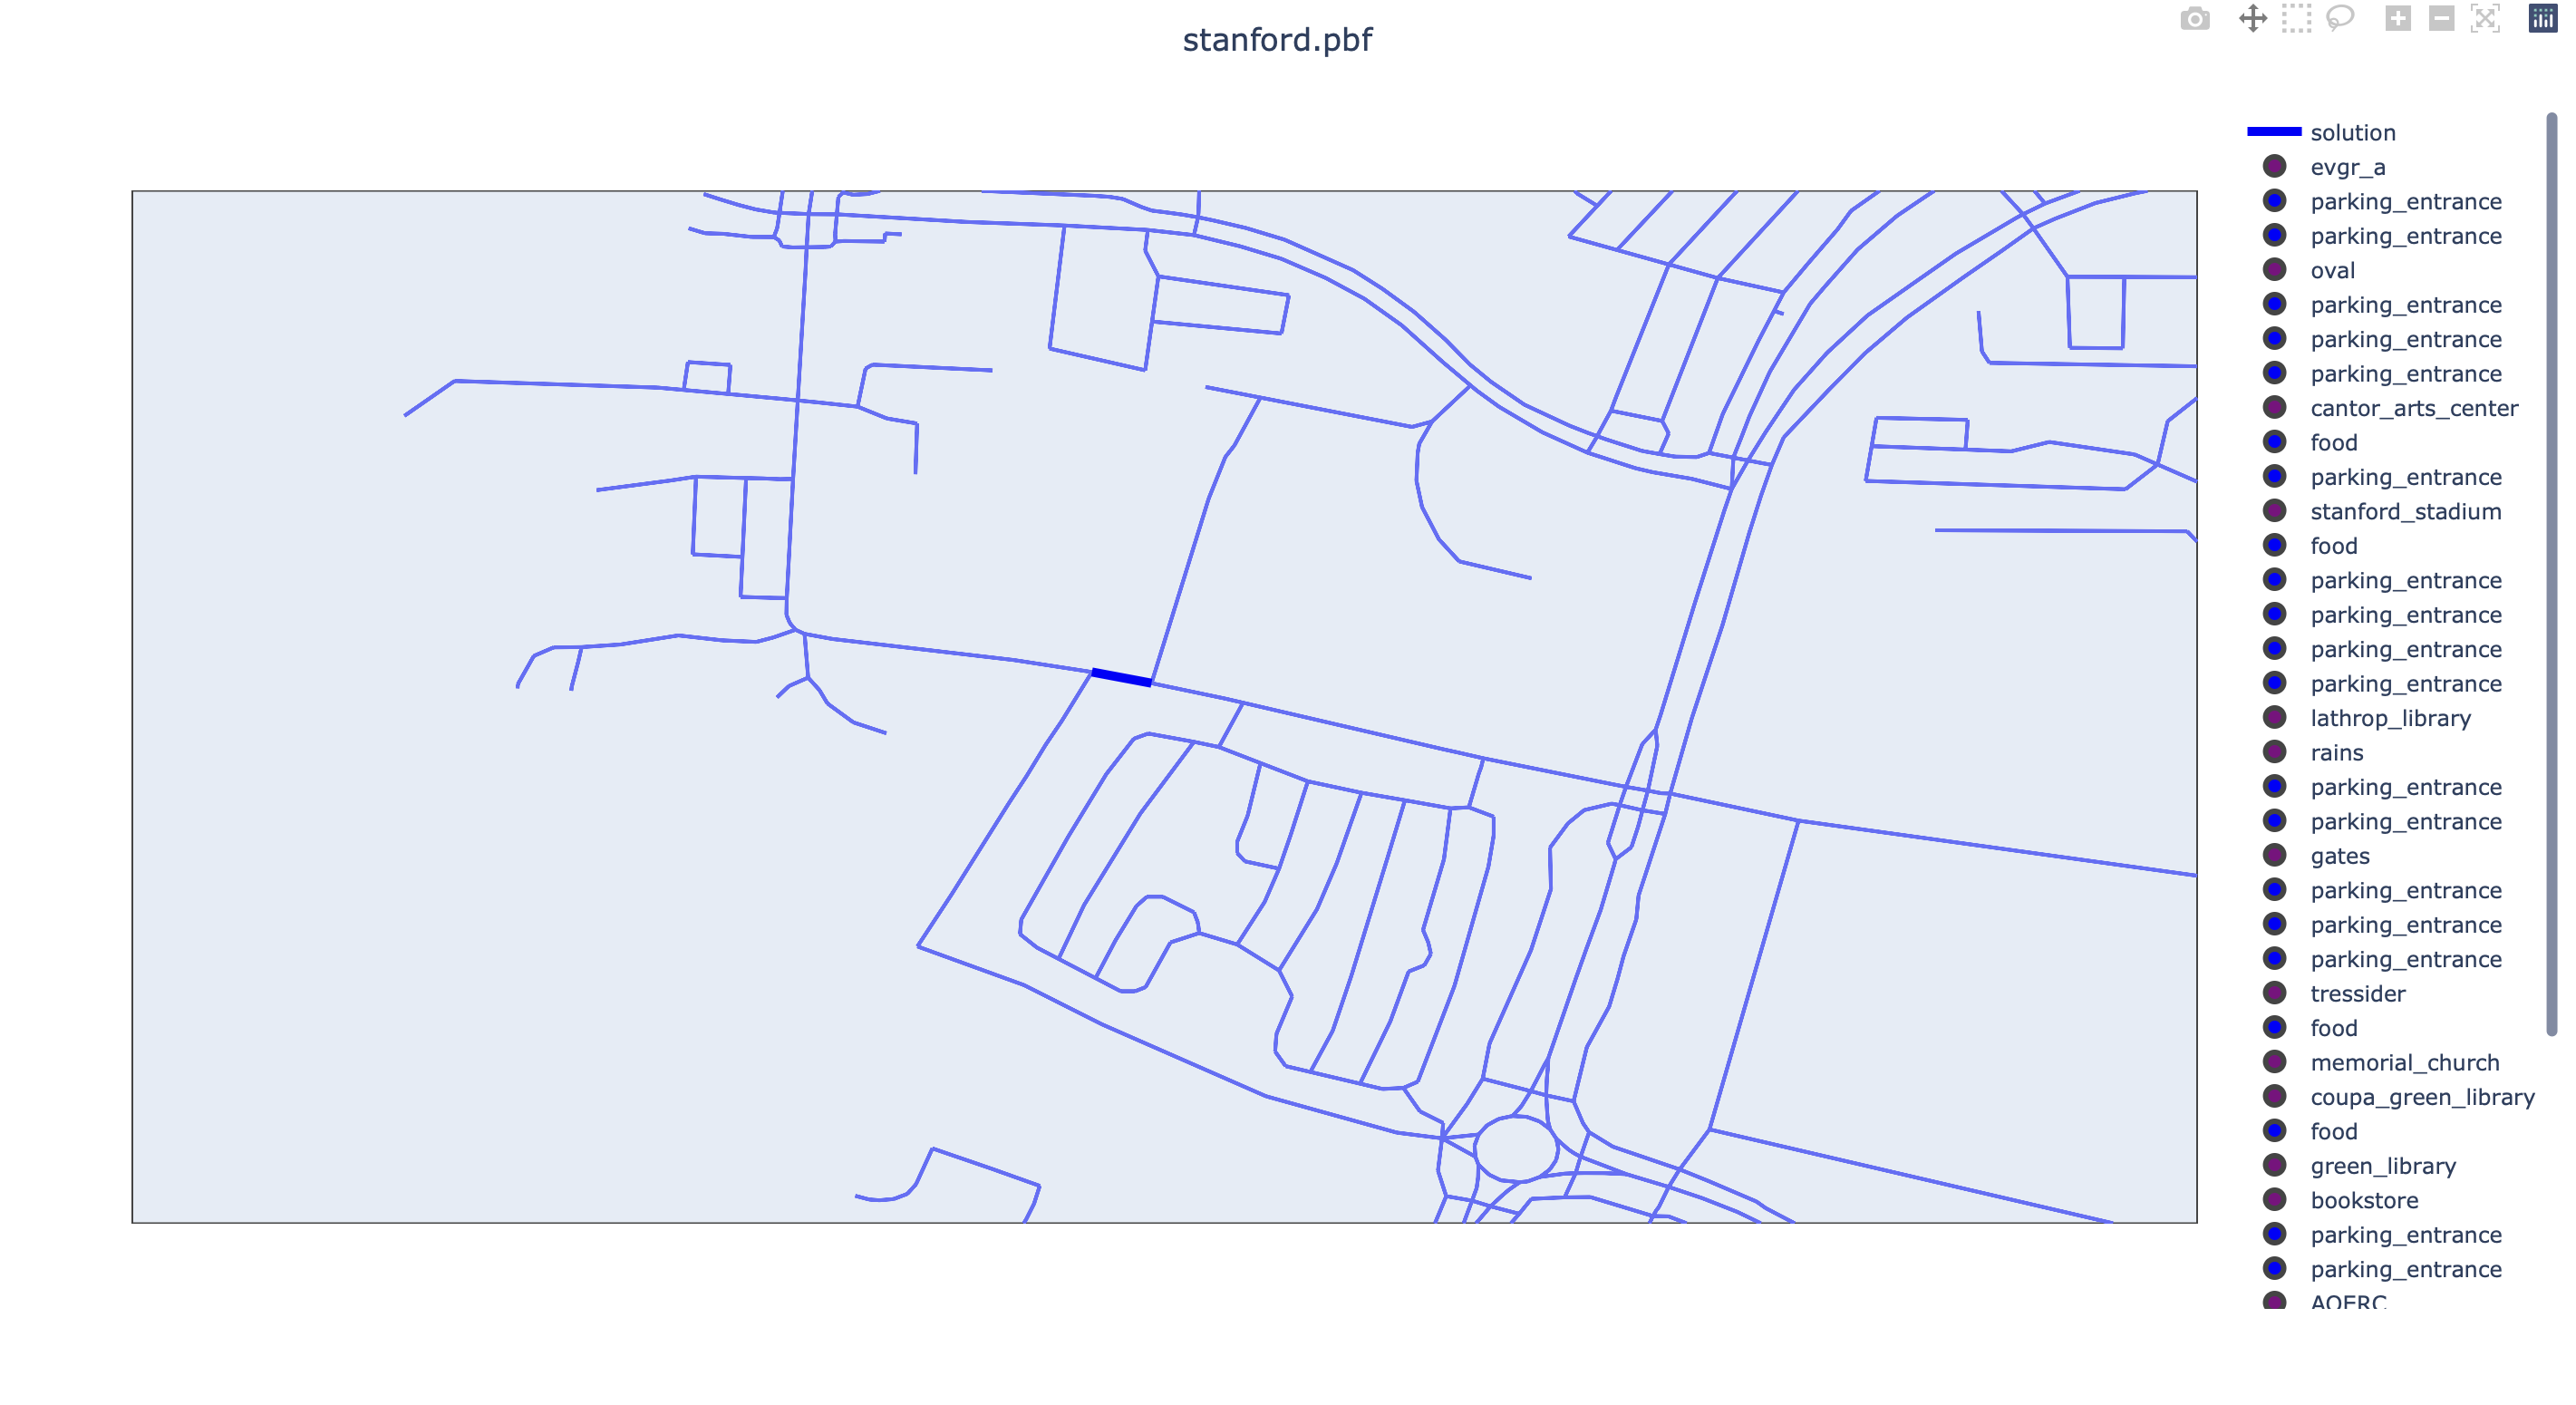
\includegraphics[width=10cm]{pics/short.png}
    \caption{startLocation='65565059', endTag="label=65422311"}
\end{figure}

可以看到这个路径非常短,原因并不是建模不正确,而是符合条件的点距离起点很近.





\section*{问题2:查找带无序途径点的最短路径(20分)}
\subsection*{a.代码实现WaypointsShortestPathProblem部分(12分)}
 \begin{lstlisting}
class WaypointsShortestPathProblem(SearchProblem):
    """The illustration and __init___ part is ommited here."""

    def startState(self) -> State:
        # BEGIN_YOUR_CODE (our solution is 1 line of code, but don't worry if you deviate from this)
        return State(location = self.startLocation, memory=self.waypointTags)
        # END_YOUR_CODE

    def isEnd(self, state: State) -> bool:
        # BEGIN_YOUR_CODE (our solution is 5 lines of code, but don't worry if you deviate from this)
        return (len(state.memory) == 0) and (self.endTag in self.cityMap.tags[state.location])
        # END_YOUR_CODE

    def successorsAndCosts(self, state: State) -> List[Tuple[str, State, float]]:
        # BEGIN_YOUR_CODE (our solution is 17 lines of code, but don't worry if you deviate from this)
        return_list = []
        succ_memory = list(state.memory)
        for tag in self.cityMap.tags[state.location]:
            if(tag in state.memory):
                succ_memory.remove(tag)
        for succ_location in self.cityMap.distances[state.location]:
            cost = self.cityMap.distances[state.location][succ_location]
            return_list.append((succ_location, State(location=succ_location, memory=tuple(sorted(succ_memory))), cost))
        return return_list
        # END_YOUR_CODE
\end{lstlisting}

\subsection*{b.回答问题(4分)}
$n\times 3^k$ 对于每一个确定的点,每个标签都有3种情况:1). 需要经过但还未经过. 2).不需要经过 3). 需要经过且已经经过 

\subsection*{c.可视化(4分)}
下面的两个路径中均有 waypointTags=['amenity=food', 'label=65559196', 'label=6524008724'].
\begin{figure}[H]
    \centering
    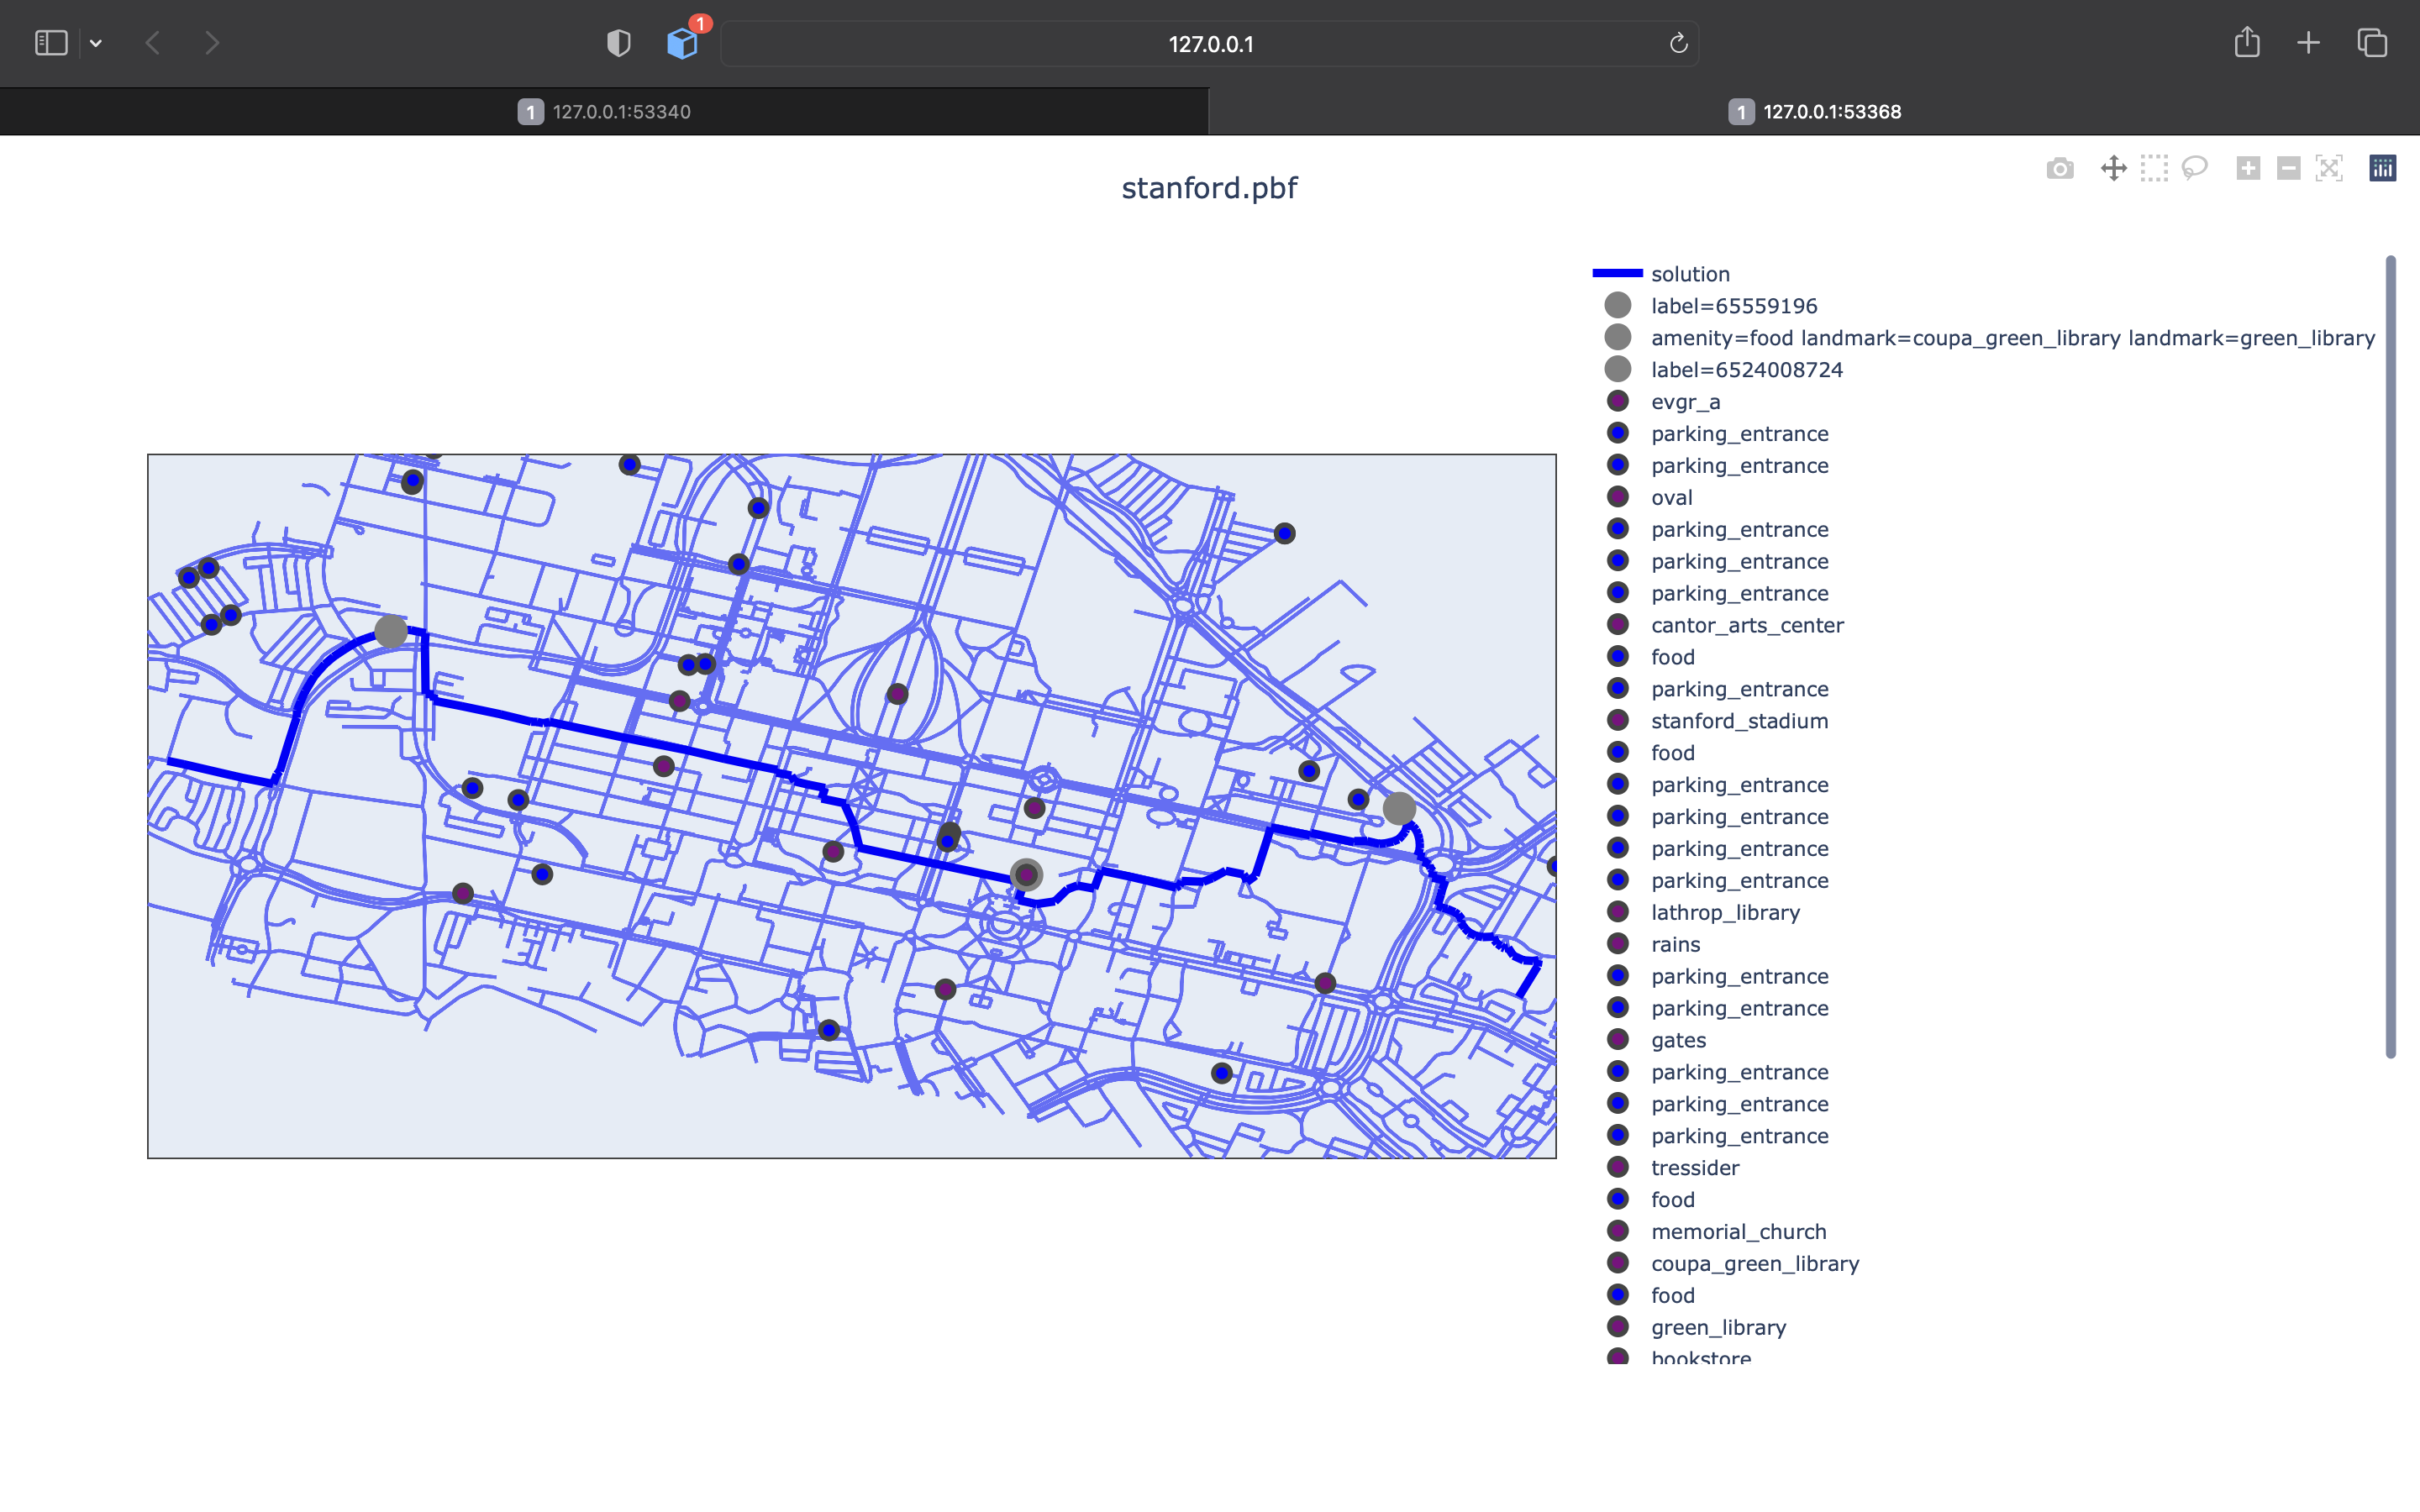
\includegraphics[width=10cm]{pics/waypoints_long.png}
    \caption{startLocation='65565059', endTag="label=9384099472"}
\end{figure}

\begin{figure}[H]
    \centering
    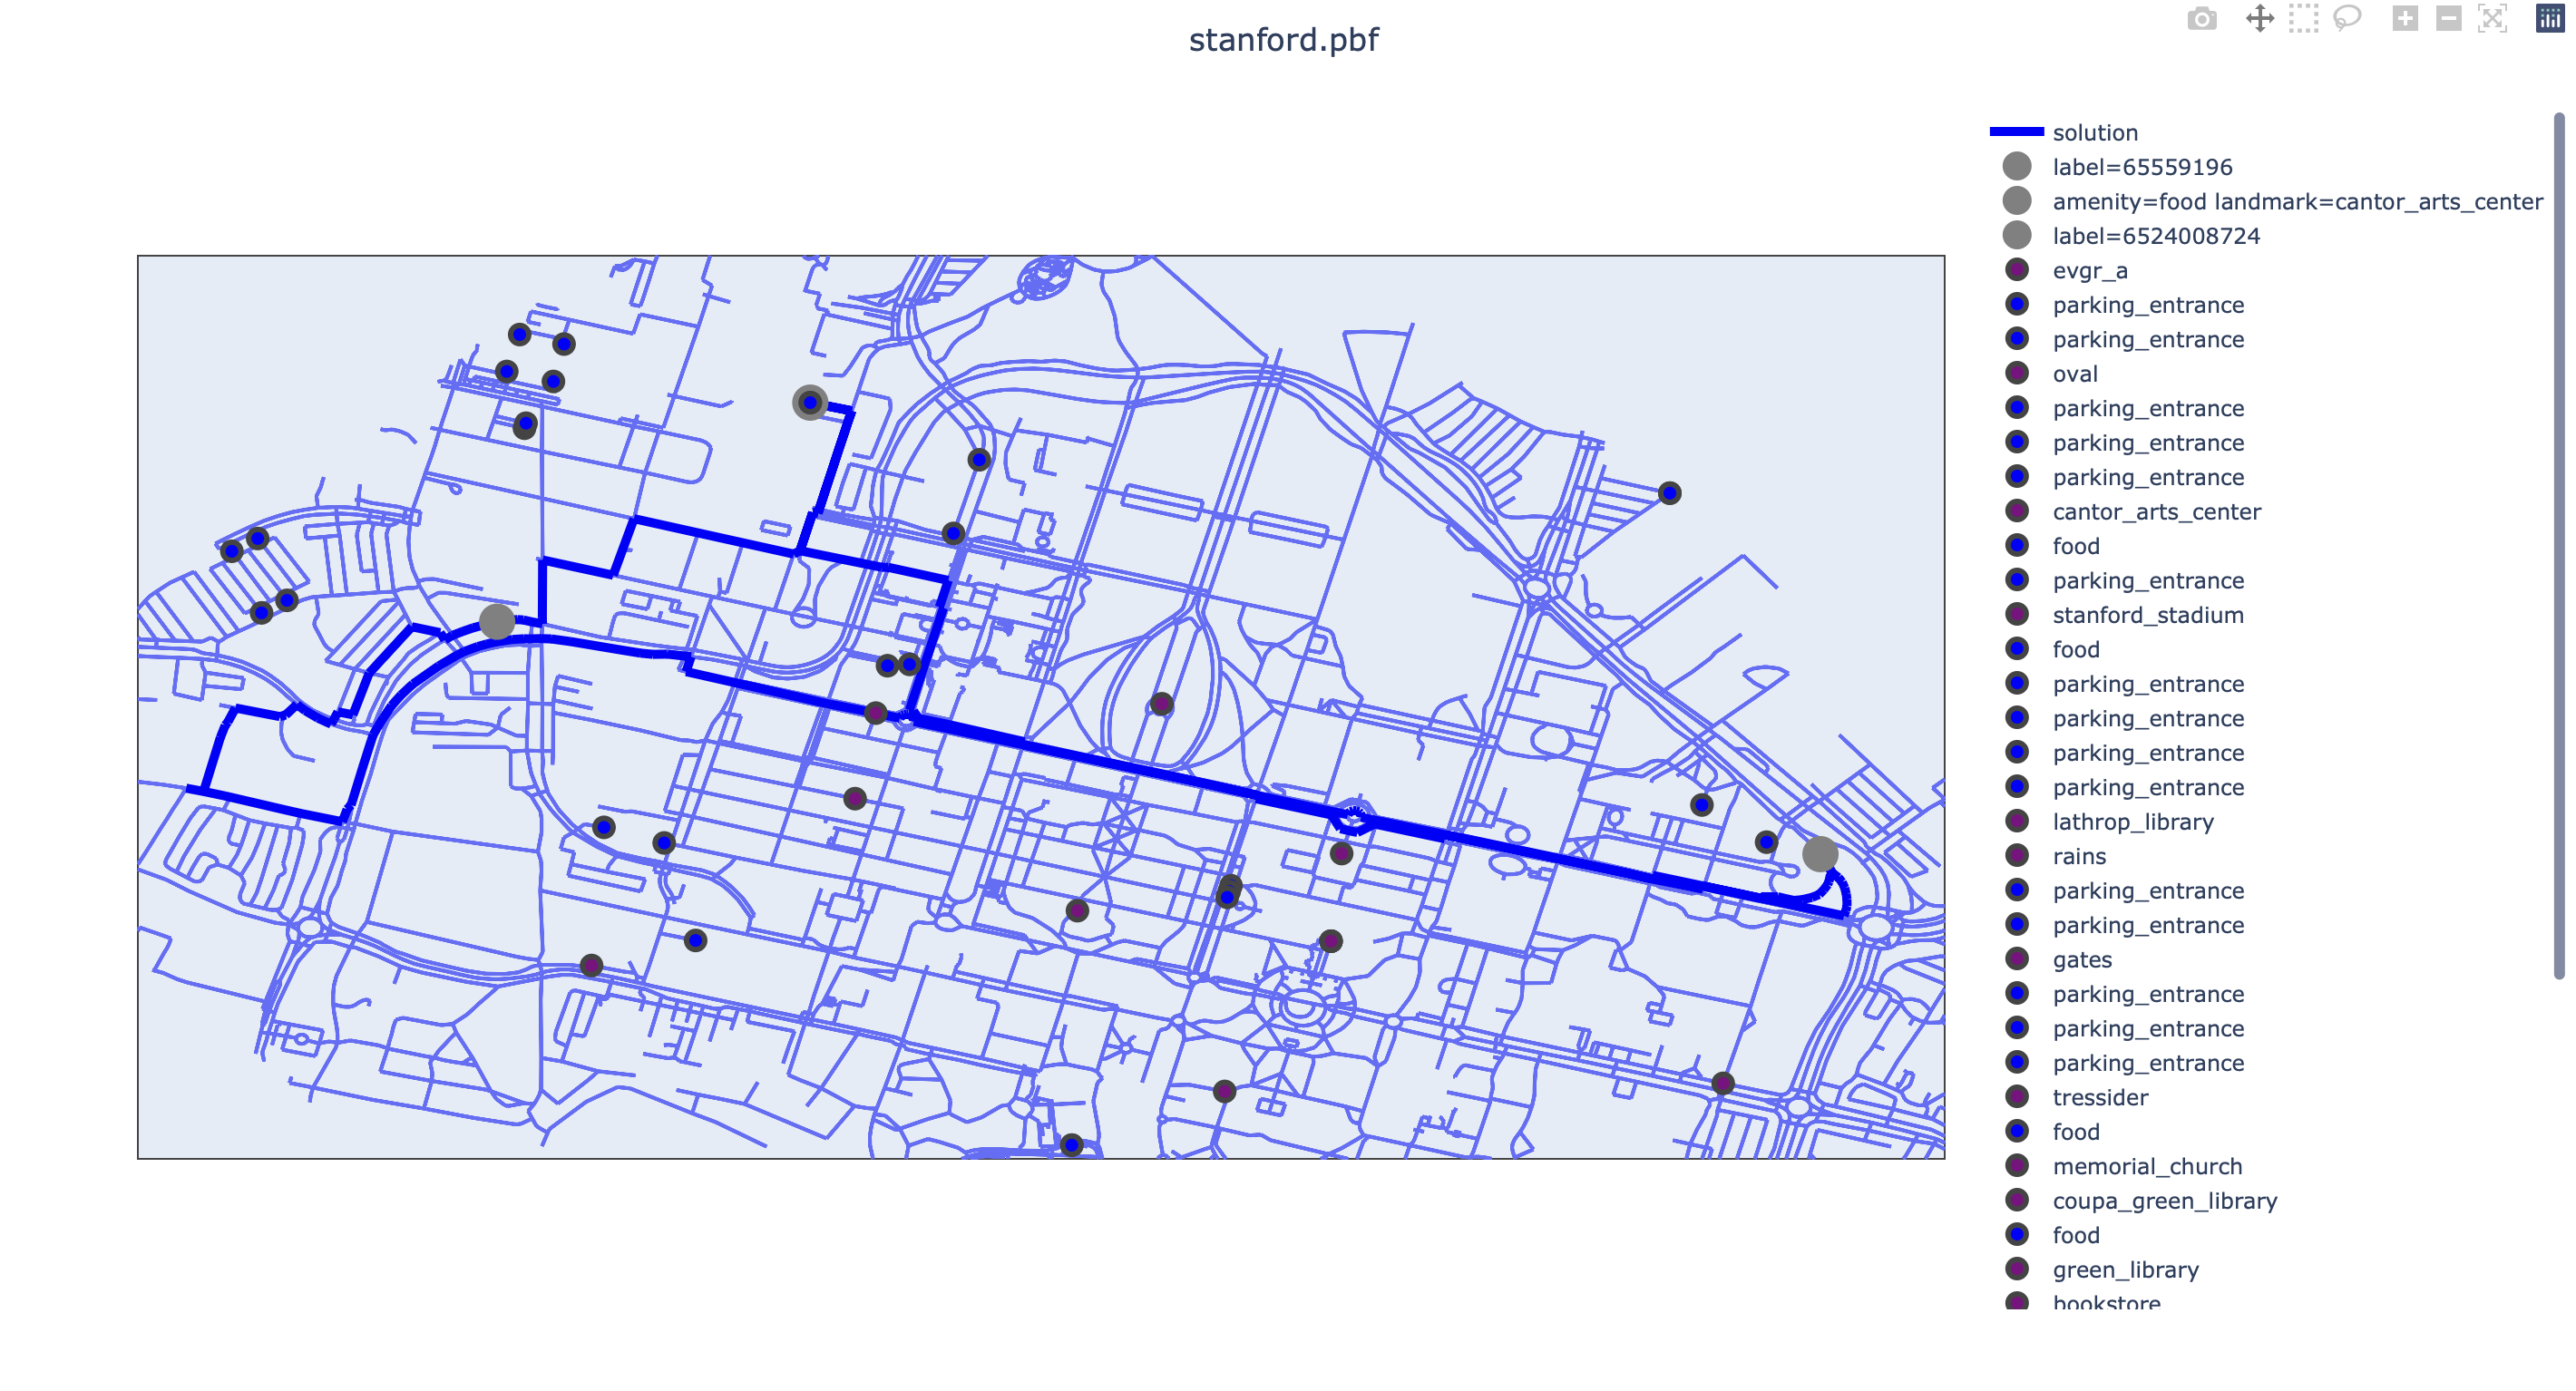
\includegraphics[width=10cm]{pics/waypoints_short.png}
    \caption{startLocation='65565059', endTag="label=65422311"}
\end{figure}

可以看到在两个路径中,设置途径点均对路径产生显著影响,使得路径可以探索更多区域.

\section*{问题3:使用 A*算法加快搜索速度(28分)}
\subsection*{a.代码实现aStarReduction的NewSearchProblem部分(8分)}
\begin{lstlisting}
def aStarReduction(problem: SearchProblem, heuristic: Heuristic) -> SearchProblem:
    class NewSearchProblem(SearchProblem):
        def startState(self) -> State:
            # BEGIN_YOUR_CODE (our solution is 1 line of code, but don't worry if you deviate from this)
            return problem.startState()
            # END_YOUR_CODE

        def isEnd(self, state: State) -> bool:
            # BEGIN_YOUR_CODE (our solution is 1 line of code, but don't worry if you deviate from this)
            return problem.isEnd(state)
            # END_YOUR_CODE

        def successorsAndCosts(self, state: State) -> List[Tuple[str, State, float]]:
            # BEGIN_YOUR_CODE (our solution is 8 lines of code, but don't worry if you deviate from this)
            org_list = problem.successorsAndCosts(state)
            return_list = []
            for tup in org_list:
                lst = list(tup)
                lst[2] += heuristic.evaluate(state)
                return_list.append(tuple(lst))
            return return_list
            # END_YOUR_CODE

    return NewSearchProblem()
\end{lstlisting}

\subsection*{b.代码实现StraightLineHeuristic部分(8分)}
\begin{lstlisting}
class StraightLineHeuristic(Heuristic):

    def __init__(self, endTag: str, cityMap: CityMap):
        self.endTag = endTag
        self.cityMap = cityMap
        # Precompute
        # BEGIN_YOUR_CODE (our solution is 5 lines of code, but don't worry if you deviate from this)
        self.endPoints = []
        for location in cityMap.geoLocations:
            if(endTag in cityMap.tags[location]):
                self.endPoints.append(location)
        # END_YOUR_CODE

    def evaluate(self, state: State) -> float:
        # BEGIN_YOUR_CODE (our solution is 6 lines of code, but don't worry if you deviate from this)
        heuristicValue = 999999999.9
        for point in self.endPoints:
            distance = computeDistance(self.cityMap.geoLocations[state.location], point)
            if(distance < heuristicValue):
                heuristicValue = distance
        return heuristicValue
        # END_YOUR_CODE
\end{lstlisting}

\subsection*{c.代码实现NoWaypointsHeuristic部分(12分)}
\begin{lstlisting}
class NoWaypointsHeuristic(Heuristic):
    
    def __init__(self, endTag: str, cityMap: CityMap):
        # Precompute
        # BEGIN_YOUR_CODE (our solution is 25 lines of code, but don't worry if you deviate from this)
        self.endPoints = []
        self.cityMap = cityMap
        self.endLocation = locationFromTag(endTag, cityMap)
        problem = ShortestPathProblem(self.endLocation, '1', self.cityMap)
        self.ucs = UniformCostSearch()
        self.ucs.solve(problem)
        # END_YOUR_CODE

    def evaluate(self, state: State) -> float:
        # BEGIN_YOUR_CODE (our solution is 1 line of code, but don't worry if you deviate from this)
        return self.ucs.pastCosts[state.location]
        # END_YOUR_CODE
\end{lstlisting}


\section*{反馈(10分)}
% 在每次实验报告的最后欢迎反馈你上这门课的感受,你可以写下任何反馈,包括但不限于以下几个方面:课堂、作业难度和工作量、助教工作等等。

\begin{itemize}
    \item 课堂体验还行
    \item 作业感觉难度有点大,花了30h+
\end{itemize}

\end{document}